\documentclass[a4paper,11pt]{article}
\usepackage{polski}
\usepackage[utf8]{inputenc}
\usepackage[OT4]{fontenc}
\usepackage{latexsym}
\usepackage{fullpage}
\usepackage{color}
\usepackage{url}
\usepackage{array}
\usepackage{graphicx}
\usepackage{listings}
\usepackage[caption=false]{subfig}

\lstset{%
	breaklines=true,
	postbreak=\raisebox{0ex}[0ex][0ex]{\ensuremath{\color{red}\hookrightarrow\space}}
}

\graphicspath{{img/}}

\title{Music OCR}
\author{
	Adam Szczepański
	\and
	Piotr Żurkowski
}

\begin{document}

\maketitle

\section{Zasada działania}

Projekt napisany jest w C++. Aby skompilować kod wystarczy wywołać komendę make.

Aby uruchomić program, należy wywołać go z parametrami plików modelu i plikiem wejściowym

\begin{lstlisting}
build/examples/piro/classification.bin NetDescriptionFile CaffeModel ImageMeanFile SynsetWordsFile InputFile
\end{lstlisting}

Przykładowy obraz \texttt{InputFile} został przedstawiony na rysunku~\ref{fig:in}.

Jako wynik, wyprodukowany zostanie plik html w folderze results. Otworzony w przeglądarce wygeneruje wizualizację nut. Przykładowy wynik został przedstawiony na rysunku~\ref{fig:out}.

\begin{figure}
\centering
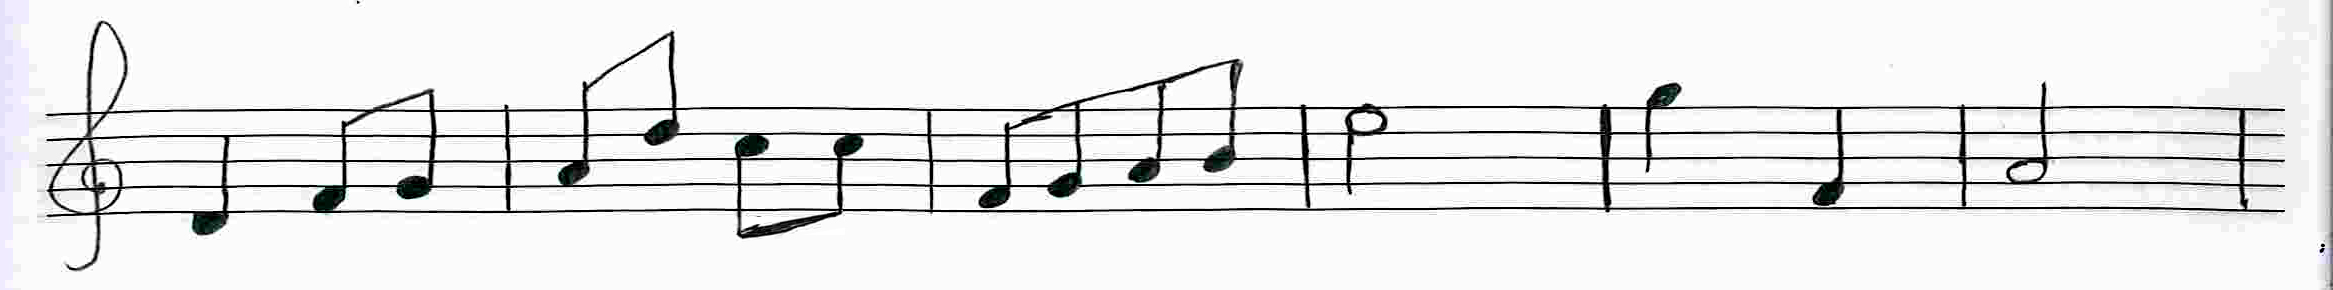
\includegraphics[width=0.8\textwidth]{in.jpg}
\caption{Obraz podawany na wejście programu}
\label{fig:in}
\end{figure}

\begin{figure}
\centering
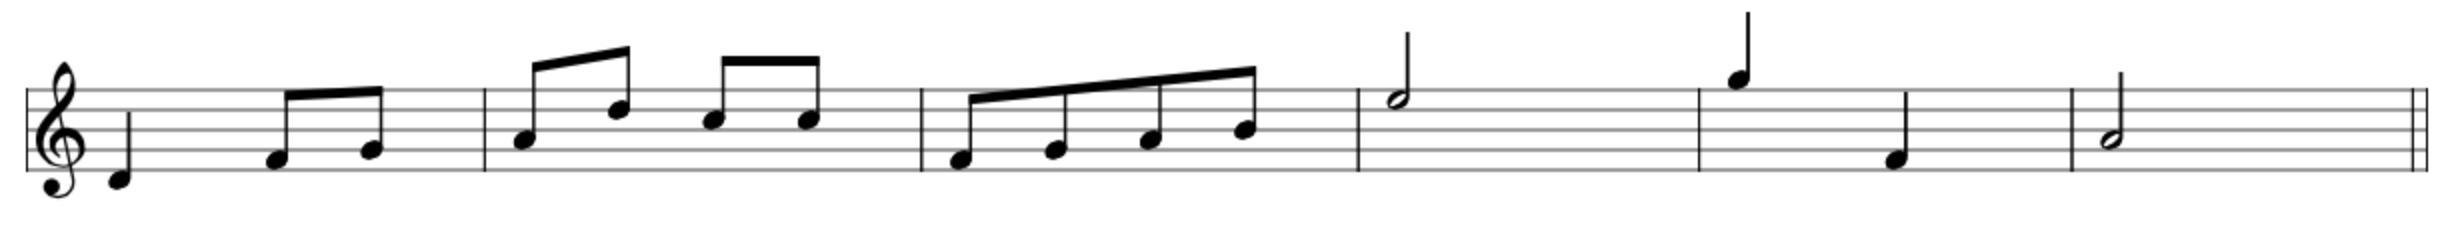
\includegraphics[width=0.8\textwidth]{out.png}
\caption{Obraz uzyskiwany na wyjściu programu}
\label{fig:out}
\end{figure}

\section{Wspierane znaki}

Algorytm wspiera poniższy zbiór symboli muzycznych
\begin{itemize}
\item Klucze
  \begin{itemize}
  \item Klucz wiolinowy
  \item Klucz basowy
  \end{itemize}
\item Nuty
  \begin{itemize}
  \item Cała nuta
  \item Półnuta
  \item Ćwierćnuta
  \item Ósemka
  \item Połączone ósemki
  \end{itemize}
\item Pauza ćwierćnutowa
\item Kreska taktowa
\end{itemize}

\section{Opis algorytmu}

Algorytm składa się z kilku kroków, zaczynając od obrazu z pojedynczą pięciolinią.
\begin{itemize}
\item Wstępne przetwarzanie obrazu
\item Wykrywanie pięciolinii i wyodrębnianie symboli z obrazu
\item Segmentacja symboli
\item Rozpoznawanie symboli
\item Wykrywanie wysokości
\item Wizualizacja
\end{itemize}

\subsection{Wykrywanie linii i nut}
Pierwszym krokiem algorytmu jest znalezienie i usunięcie pięciolini z obrazu.
Po wstępnym thresholdowaniu i zmiany obrazu na binarny, wywoływana jest erozja i dylatacja, z kernelem w postaci macierzy 1 x width/30.
w ten sposób na obrazie zostają tylko poziome linie.
Podobna operacja wykonywana jest też wertykalnie, aby wspomóc proces ekstrakcji znaków opisany dalej.

Wyodrębniane linie, po dodatkowej dylatacji pionowej, odejmowane są od orginalnego obrazu.
W celu poprawy wyniku dodaje się wyodrębnione wcześniej elementy wertykalne.
Następnie obraz jest ponownie progowany, prowadząc do obrazu zawierającego same nuty. Przykładowy efekt usuwania linii został przedstawiony na rysunku~\ref{fig:notes}.

W międzyczasie, wyekstraktowane linie przetwarzane są w celu znalezienia głównych pięciu, wykorzystywanych do szacowania wysokości.
Na obrazie sumowane są pixele w każdym wierszu, i progowane 30\% maksymalnej wartości.
W ten sposób otrzymywani są kandydaci na pięciolinię. następnie bliscy kandydaci łączeni są w jednych, po czym wybierane jest 5 najwyższych wartości.
Pozycje linii są zapisane, wraz ze średnią odległością między liniami.

\begin{figure}
\centering
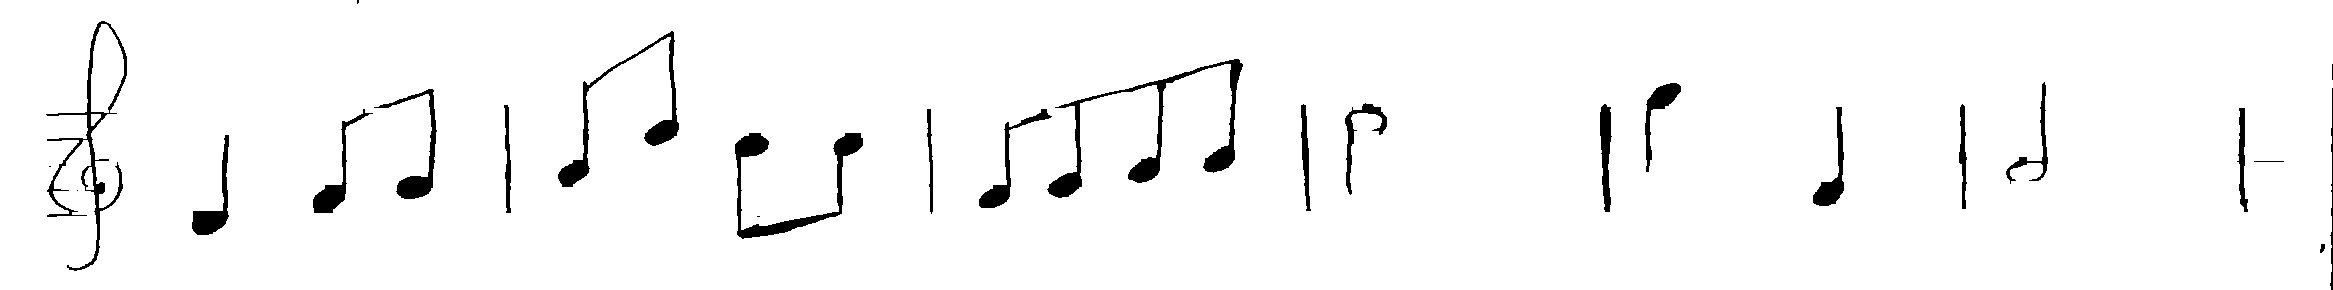
\includegraphics[width=0.8\textwidth]{notes.jpg}
\caption{Wycięte linie}
\label{fig:notes}
\end{figure}

\subsection{Segmentacja nut}
Segmentacja nut przeprowadzana jest na wyekstraktowanych symbolach z poprzedniego kroku.
Dla każdej kolumny sprawdzana jest zawartość czarnych pixeli i grupowane są kolejne kolumny które takie pixele zawierają.
Następnie łączone są grupy odległe o mniej niż połowa szerokości linii - w ten sposób unikając błędów wynikających z niedokładnych skanów lub niedokładnie narysowanych nut.
Jako wynik otrzymujemy listę grup w postaci zakresów kolumn, w których mogą znajdować się symbole.

Jako kolejny krok, wykonywane jest sprawdzenie, czy grupa zawiera pojedynczy symbol, czy połączoną grupę nut.
Przy obserwacji, że połączone nuty zawsze są pełne w środku, można podjąć się szukania główek nut w grupach jako wyznacznik czy grupa jest pojedynczym symbolem czy grupą nut.

Wyszukiwanie główek nut, odbywa się poprzez znalezienie w każdej kolumnie najdłuższego ciągu czarnych pixeli.
Kandydatami są ciągi o długości większej niż połowa wysokości linii, i mniejszej niż półtora wysokości linii.
kandydaci grupowani są w grupy, jeśli są odległe od siebie nie więcej niż 2 pixele (dopuszczenie szumów).
Kandydatami pozostają grupy, które są szerokie na przynajmniej połowę szerokości linii.
W ten sposób otrzymujemy listę możliwych główek nut.  Jeśli lista zawiera więcej niż jedną główkę nuty, jest traktowana jako połączone nuty.
Jeśli nie, traktowana jest jako pojedynczy symbol. Pojedyncze symbole przechodzą do fazy rozpoznawania i wykrywania wysokości.
Połączone traktowane są jako ósemki i przechodzą bezpośrednio do fazy wykrywania wysokości.
Wynik segmentacji nut został przedstawiony na rysunku~\ref{fig:argb}.

\begin{figure}
\centering
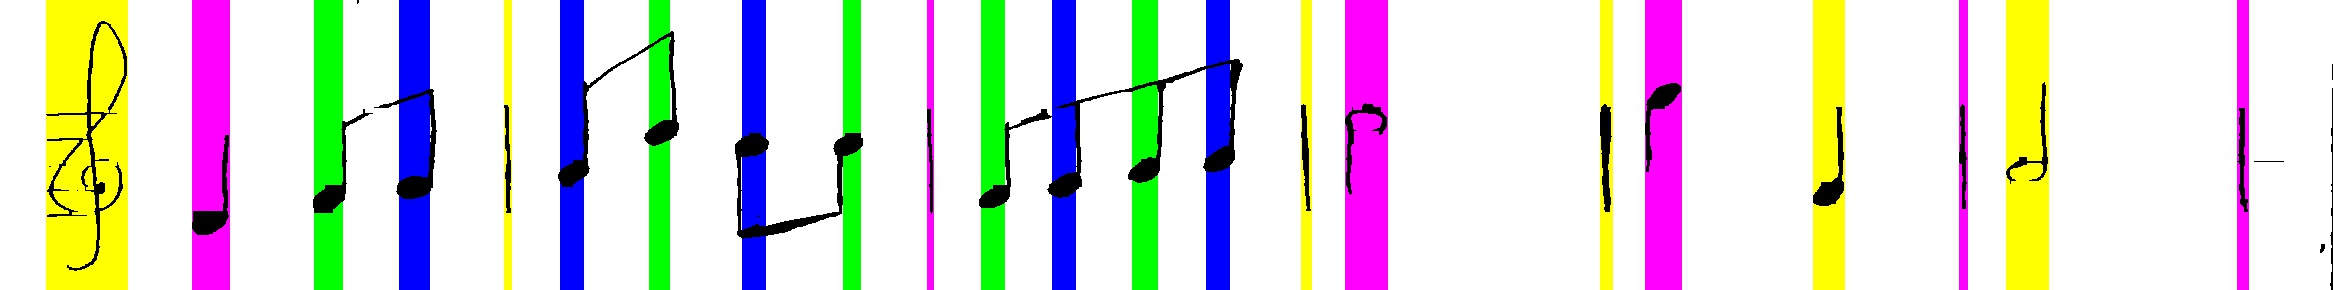
\includegraphics[width=0.8\textwidth]{argb.jpg}
\caption{Wynik segmentacji. Żółte i fioletowe segmenty oznaczają pojedyncze nuty. Niebieskie i zielone oznaczają główki nut połączonych.}
\label{fig:argb}
\end{figure}


\subsection{Rozpoznawanie symboli}

Do rozpoznawania nut wykorzystano \emph{caffe} -- framework deep learning~\cite{jia2014caffe} rozwijany przez \emph{Berkeley Vision and Learning Center}. Platforma umożliwia szybkie i~modularne uczenie modeli w~oparciu o~sieci opisane w~plikach tekstowych i~przygotowane zbiory treningowy i~walidujący z~obrazkami.

Przygotowano zbiór uczący składający się z~341 obrazków i~zbiór walidujący składający się z~274 obrazków. Oba zbiory zawierają zarówno znaki drukowane jak i~pisane ręcznie. Liczności poszczególnych znaków znajdują się w~tabeli~\ref{tab:train_val}. Przykładowe rozpoznawane znaki znajdują się na rysunku~\ref{fig:crops}.

\begin{table}
\centering
\begin{tabular}{l|c|c}
znak & zbiór uczący & zbiór walidujący \\ \hline
Klucz wiolinowy & 40 & 22 \\
Klucz basowy & 40 & 29 \\
Cała nuta & 40 & 34 \\
Półnuta & 41 & 33 \\
Ćwierćnuta & 40 & 40 \\
Ósemka & 50 & 35 \\
Pauza ćwierćnutowa & 40 & 31 \\
Kreska taktowa & 50 & 50 \\ \hline
razem & 341 & 274 \\
\end{tabular}
\caption{Liczności zbiorów uczących i~walidujących.}
\label{tab:train_val}
\end{table}

Przed rozpocząciem procesu uczenia wszystkie obrazki zostały przekonwertowane do odcieni szarości, przeskalowane do rozmiarów 256x256 i~zgromadzone w jednej bazie danych wspieranej przez \emph{caffe} oraz obliczona została ich średnia jasności obrazów. Wykorzystana sieć neuronowa składa się z~8 głównych warstw ukrytych.

Warstwa wejściowa pobiera obrazy z~bazy danych. Następnie 5~warstw konwolucyjnych -- splatająca obraz który otrzymuje na wejściu ze zbiorem masek podlegających uczeniu, z~których każda produkuje osobny wynik wykorzystywany w~kolejnej warstwie. Pomiędzy warstwami konwolucyjnymi występują warstwy normalizujące, ReLU (zwracające \emph{max(x,0)} oraz MaxPooling (wybierające dla rozłącznych regionów maksymalne wartości). Następnie w~sieci znajdują się 3~warstwy w~pełni połączone -- traktujące wejście jako wektor i~dające na wyjściu wektor. Pomiędzy tymi warstwami znajdują się warstwy normalizującem ReLU oraz Dropout (odrzucająca część danych podczas uczenia). Warstwa wyjściowa zwraca dla każdego rozpoznawanego znaku prawdopodobieństwo, że klasyfikator zaklasyfikował obrazek jako ten znak.

Wykorzystane zostały parametry uczenia:
\begin{itemize}
\item Prędkość uczenia: 0.01
\item Momentum: 45000
\item Weight decay: 0.0005
\end{itemize}

Model był zapisywany do pliku co 50 iteracji i~był testowany co 100 iteracji. Otrzymany po 1800 iteracjach model daje trafność 95.9\% na zbiorze walidującym.

Wykorzystana sieć wzorowana była na~\cite{NIPS2012_4824}.

\subsection{Wykrywanie wysokości}
Dla wyciętego już obrazu nuty, wyszukuje się prawdopodobnej pozycji na pięciolinii.
Na początku przetwarzania, liczy się przedziały przynależności nut do wysokości.
Dla wcześniej wyznaczonych pozycjii pięciu linii, zapisywane są przedziały przynależności - dla położenia na linii -
$<PozycjaLinii - 0.25 * SzerokośćLinii, PozycjaLinii + 0.25 * SzerokośćLinii>$ - dla położenia pomiędzy liniami -
$<PozycjaDolnejLinii + 0.25 * SzerokośćLinii, PozycjaGórnejLinii - 0.25 * SzerokośćLinii>$.
Analogicznie szacowane są pozycje nut poniżej i powyżej pięciolinii.

Następnie dla nuty, liczone są pixele w każdym rzędzie, thresholdowane 30\% maksymalnej wartości, i grupowane w spójne przedziały.
Znajdowany jest najdłuższy przedział i jest traktowany jako główka nuty
(Wybrano najdłuższy przedział a nie najgęstrzy segment, ponieważ półnuty są puste w środku i mogą być łatwo przewyższone szumem z innych miejsc).
Dla znalezionego już przedziału, liczy się środek ciężkości jako wyznacznik położenia nuty.

Mając przewidywane położenie nuty, sprawdza się przynależność do przedziałów i przypisuję wysokość nucie.

\begin{figure}[!bt]
\centering
\subfloat[klucz wiolinowy]{
	\hspace*{16pt}
	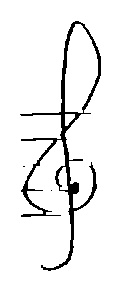
\includegraphics[width=0.08\textwidth]{crop_tc.jpg}
	\hspace*{16pt}
}\hfill
\subfloat[klucz basowy]{
	\hspace*{16pt}
	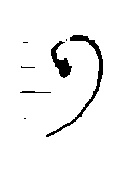
\includegraphics[width=0.08\textwidth]{crop_bc.jpg}
	\hspace*{16pt}
}\hfill
\subfloat[kreska taktowa]{
	\hspace*{16pt}
	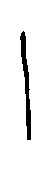
\includegraphics[width=0.08\textwidth]{crop_bar.jpg}
	\hspace*{16pt}
}\hfill
\subfloat[pauza]{
	\hspace*{16pt}
	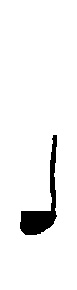
\includegraphics[width=0.08\textwidth]{crop_n4.jpg}
	\hspace*{16pt}
} \\
\subfloat[cała nuta]{
	\hspace*{16pt}
	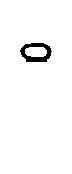
\includegraphics[width=0.08\textwidth]{crop_n1.jpg}
	\hspace*{16pt}
}\hfill
\subfloat[półnuta]{
	\hspace*{16pt}
	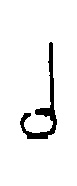
\includegraphics[width=0.08\textwidth]{crop_n2.jpg}
	\hspace*{16pt}
}\hfill
\subfloat[ćwierćnuta]{
	\hspace*{16pt}
	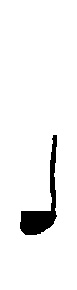
\includegraphics[width=0.08\textwidth]{crop_n4.jpg}
	\hspace*{16pt}
}\hfill
\subfloat[ósemka]{
	\hspace*{16pt}
	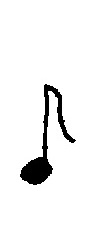
\includegraphics[width=0.08\textwidth]{crop_n8.jpg}
	\hspace*{16pt}
}
\caption{Rozpoznawane znaki}
\label{fig:crops}
\end{figure}

\subsection{Wizualizacja}
Do wizualizacji wykorzystywana jest biblioteka VexFlow, pozwalająca na renderowanie pięciolinii w przeglądarce, za pomocą JavaScript.
Kod generuje gotowy plik html, z kodem w JS generujący gotową pięciolinię.
Wygenerowane nuty, mogą wizualnie różnić się od tych czytanych,
np. pionowa kreska nuty może być skierowana w dół a nie w górę, itd. ponieważ algorytm rysowania sam dobiera takie parametry.
Merytorycznie jednak, wygenerowane nuty mają takie same znaczenie.

\section{Wyniki testów}
Testy przeprowadzono na ponad 600 nutach narysowanych odręcznie. Wyniki przedstawione są poniżej.
Widać spory problem z segmentacją całych nut i półnut, spowodowany problemami z wycinaniem dolnych części nut w pewnych przypadkach.
Problemy z segmentacją występują również dla ósemek, które spowodowane są głównie przerywanymi połączeniami między nutmami.
Przy klasyfikacji główny problem pojawia się w przypadku klucza basowego - spowodowanego wycinaniem górnej części klucza w większości przypadków -
oraz dla pauz - które w formie odręcznej różnią się między sobą znacząco.

\begin{table}[!ht]
\centering
\begin{tabular}{|r|r|r|r|}
\hline
Znak | Błąd & bł. segmentacji & bł. klasyfikacji & bł. wykr. wysokości \\ \hline
Klucz wiolinowy & 1.6\% & 4.8\% & - \\
Klucz basowy & 2.9\% & 10.8\% & - \\
Cała nuta & 20.2\% & 5.5\% & 5.4\%\\
Półnuta & 9.6\% & 5.4\% & 6.7\% \\
Ćwierćnuta & 0\% & 2.5\% & 1.3\% \\
Ósemka & 9.4\% & 3.5\% & 10.5\% \\
Pauza ćwierćnutowa & 7\% & 14.1\% & - \\
Kreska taktowa & 2\% & 8\% & - \\ \hline

\end{tabular}
\caption{Procent błędów każdego typu, dla wszystkich rozpoznawanych znaków.}
\label{tab:test_results}
\end{table}



\bibliography{report}
\bibliographystyle{plain}

\end{document}
